\chapter{Event Reconstruction}

\label{ch:reconstruction}
% --------------------------------------------------------------------------------

The ATLAS experiment combines measurements in the subdetectors to form a cohesive picture of each physics event. 
The majority of particles that traverse the detector leave behind some combination of ionization hits in the tracking detectors or energy deposits in the calorimeters, and these measurements can be used to reconstruct physical quantities like the particle's energy, momentum, or trajectory.
Even the type of the particle can be distinguished by comparing the various ways that different species of stable particles interact with the subdetectors.
Reconstruction is the series of algorithms which take the electronic outputs of the detector and assigns them into individual physics objects.
The physics objects summarize the properties of particles produced by the collision or subsequent decays, either for individual isolated particles like leptons, or for a collection of the cascade of products produced in the decay of an energetic hadron, called a jet. 
These are the objects and quantities most often used in analysis to make measurements of \ac{SM} processes or to search for new physics.

% ----------------------------------------

\section{Charged Particles}
\label{sec:tracks}

As described in Section~\ref{sec:inner_detector}, charged particles that traverse the inner detector leave behind hits in the subdetectors.
Each of these hits translates into a position measurement along the trajectory of that particle, with position resolutions depending on the subdetector that provided the measurement. 
Track reconstruction uses these position measurements to collect hits in consecutive layers of the detector into a trajectory consistent with a particle curving in a magnetic field~\cite{newt, tracking_performance}.
This reconstructed trajectory is called a track.
The number of hits in the inner detector for each event makes a combinatorial method completely infeasible: the algorithms that form tracks must be significantly more intelligent so that event reconstruction does not exhaust computing resources.

The first and primary algorithm employed in track reconstruction is called the inside-out method, which begins with the assumption that the track originated from the interaction point.
Its purpose is to identify primary particles, those which originate in the proton-proton collisions and with a lifetime long enough to reach the inner detector.
Combinations of three hits are considered from measurements in the Pixel detector and the \ac{SCT}, and form the seed for a track. 
Specifically, the seeding algorithm looks for a seed using three pixel hits, two pixel hits and one \ac{SCT} hit, or three \ac{SCT} hits.
The seed is then extrapolated forwards and backwards into the Pixel and \ac{SCT} detectors depending on the seed location, and hits in each layer are considered to be added to the track using a combinatorial Kalman filter~\cite{tracking_performance}.
After all of the silicon layers have been considered, tracks are filtered to reduce ambiguities from other nearby tracks or from combinatorial coincidences.
Then the tracks are extended outwards into the \ac{TRT} in the same way.
This algorithm is how the hits are chosen to be incorporated into a single track.
Once the hits are collected, a fitting algorithm calculates the track parameters which best model the locations of the hits and their resolutions.
The fitting uses five parameters, $(d_0, z_0, \phi, \theta, q/p)$, to specify a track in a perigee representation: $d_0$ and $z_0$ are the transverse and longitudinal impact parameters at the closest approach to the nominal beam axis, $\phi$ and $\theta$ are the usual angular coordinates, and $q/p$ is the charge divided by the momentum.
These parameters are illustrated in Figure~\ref{fig:perigee_rep}.
Those parameters directly determine the direction and momentum of the particle which produced the track.

\begin{figure}
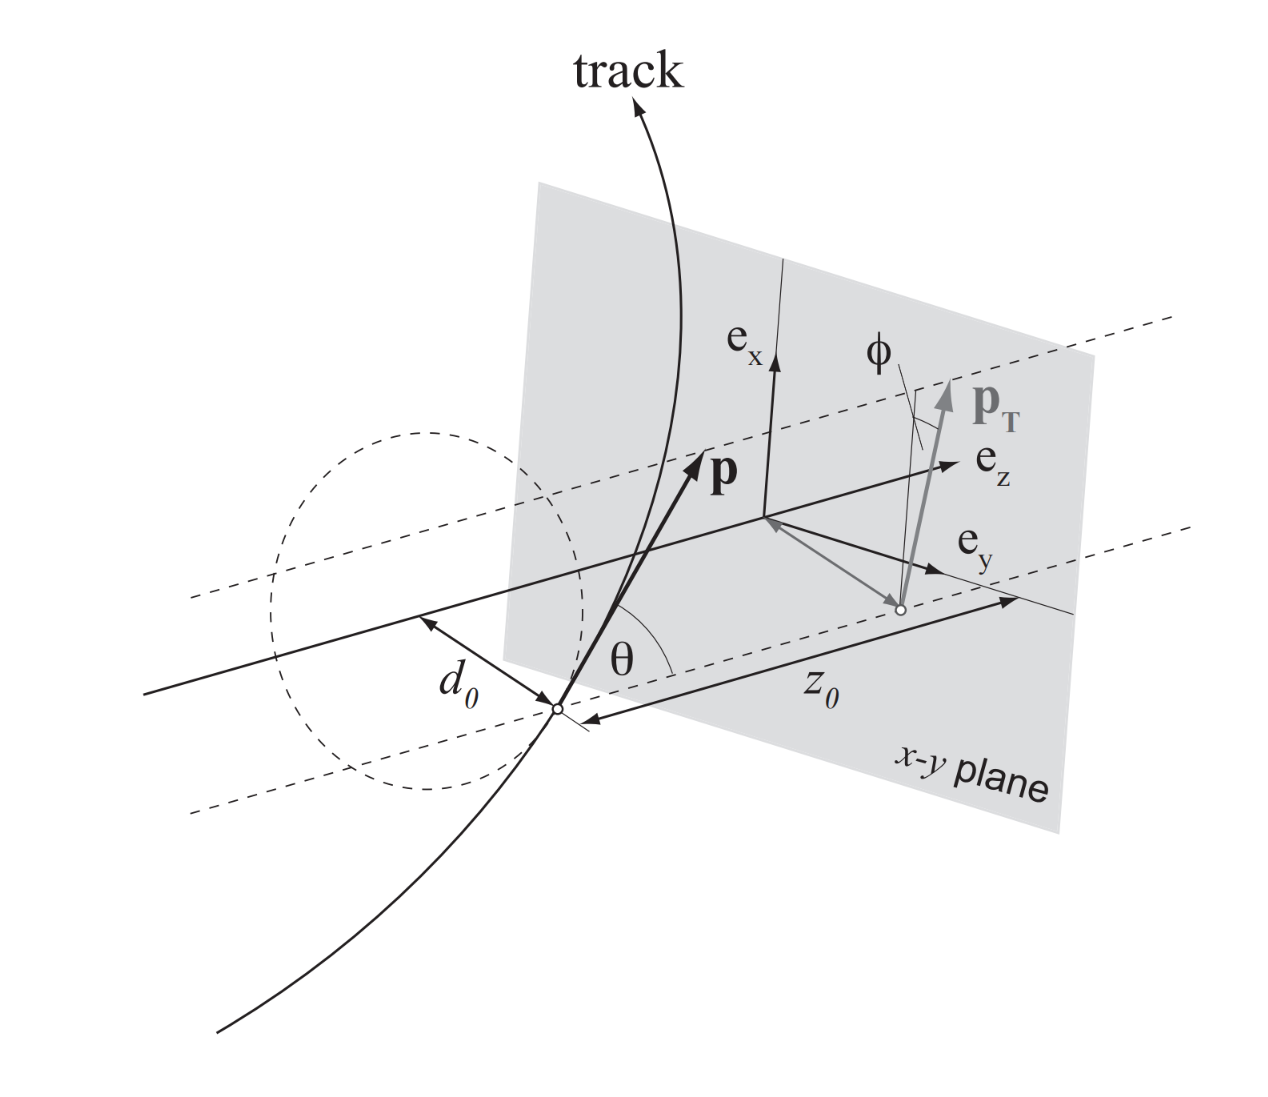
\includegraphics[width=\fullfig]{figures/perigee_rep.png}
\caption{An illustration of the perigee representation of track parameters for an example track. The charge is not directly shown, but is indicated by the direction of curvature of the track~\cite{atlas_extrapolation}.}
\label{fig:perigee_rep}
\end{figure}

This inside-out algorithm is complemented by an outside-in algorithm, which is used to find tracks from secondary particles, those produced in the decays or interactions of the primary particles inside the detector. 
As the name indicates, the outside-in algorithm begins by seeding tracks in the outermost layers of the inner detector, in the \ac{TRT}. 
The seed in this case is formed by a segment in the \ac{TRT}, and the track is propagated backwards into the \ac{SCT} before being refitted to use all the included points.
Some tracks are found with \ac{TRT} segments only, which can result from interactions with the detector following the \ac{SCT}.
Figure~\ref{fig:track_patterns} shows an example of the geometry of tracks formed by both algorithms, where the hits belonging to tracks found using the inside-out algorithm are highlighted in red, and the hits belonging to the tracks found using the outside-in algorithm are circled in black.
The figure highlights the presence of a large number of both primary and secondary tracks in a single event, as well as the overall large number of hits present in the inner detector.

\begin{figure}
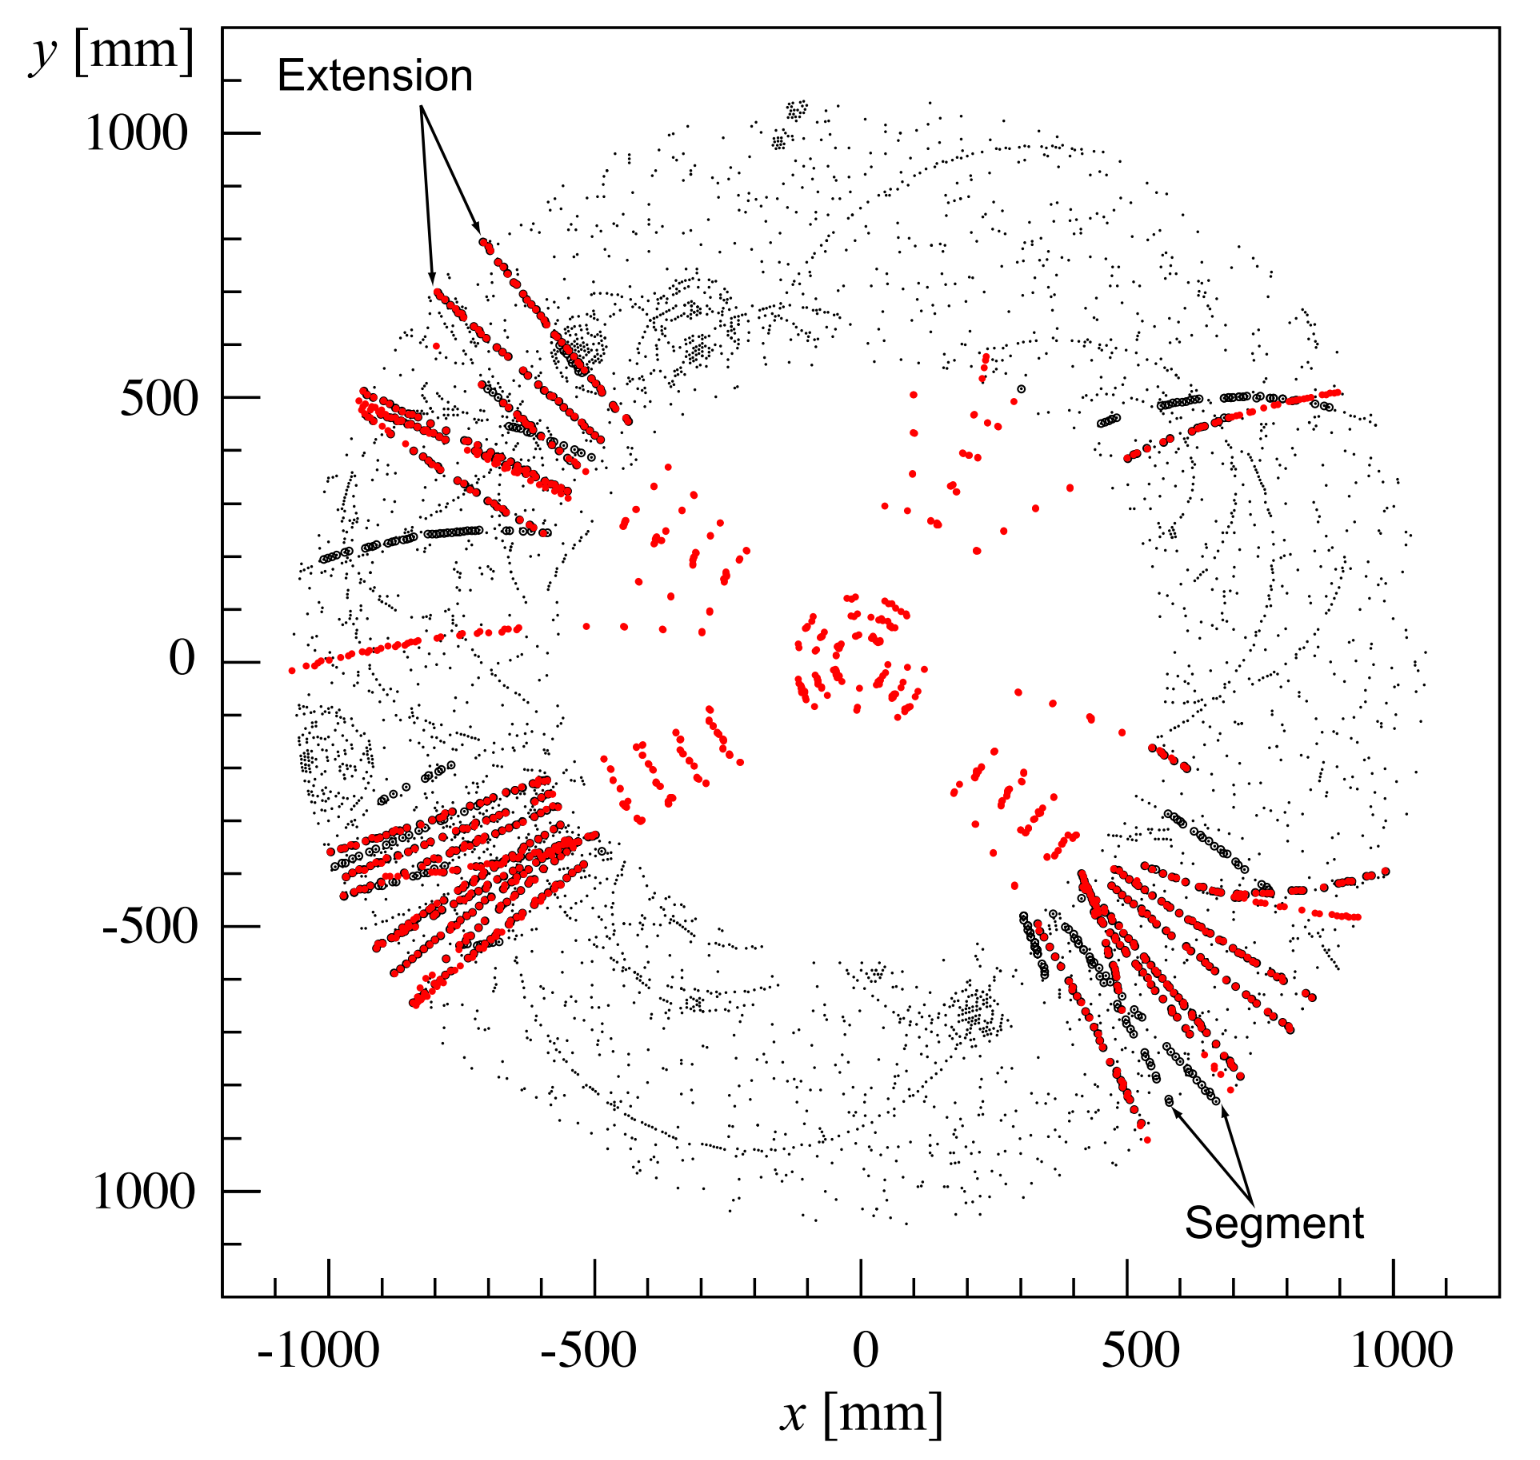
\includegraphics[width=\fullfig]{figures/track_patterns.png}
\caption{The $x$ and $y$ locations of the hits generated in a simulated $t\bar{t}$ event in the inner detector. The hits which belong to tracks formed using the inside-out algorithm are highlighted in red, while the hits which belong to tracks formed using the outside-in algorithm are circled in black.}
\label{fig:track_patterns}
\end{figure}

The tracks resulting from these algorithms can be contaminated by nearby particles confusing the tracking algorithm in a high luminosity environment.
For example, enough hits present in the inner detector can lead to fake tracks from combinations of hits from multiple individual tracks.
Therefore, after the tracks are formed and fitted, additional quality requirements are imposed in order to reduce such backgrounds.
Most tracking applications require at least seven silicon hits, that is, seven hits between the Pixel detector and \ac{SCT}.
Then the tracks are required to have at most two holes in the Pixel detector, where holes are non-existing but expected measurements in a layer of the subdetector.
If the missing hit corresponds to an inactive module, however, it is not counted as a hole but instead as a hit for tracking as the lack of a measurement is expected in that case.

\subsection{Pixel Neural Network}

The hits in the Pixel detector are not typically confined to a single pixel, but rather the charge is spread over several pixels per layer which are grouped together into clusters.
The clustering of these pixels for isolated tracks is relatively straightforward, but complications can arise in the high occupancy environment where hits from multiple particles can overlap in a single cluster.
Figure~\ref{fig:pixel_cluster_types} shows examples of clusters generated by a single isolated particle, two nearly overlapping particles, and a particle which emits a $\delta$-ray. 
A $\delta$-ray is a secondary electron which is generated with enough energy to escape a significant distance away from the original particle and to generate additional ionization.

\begin{figure}
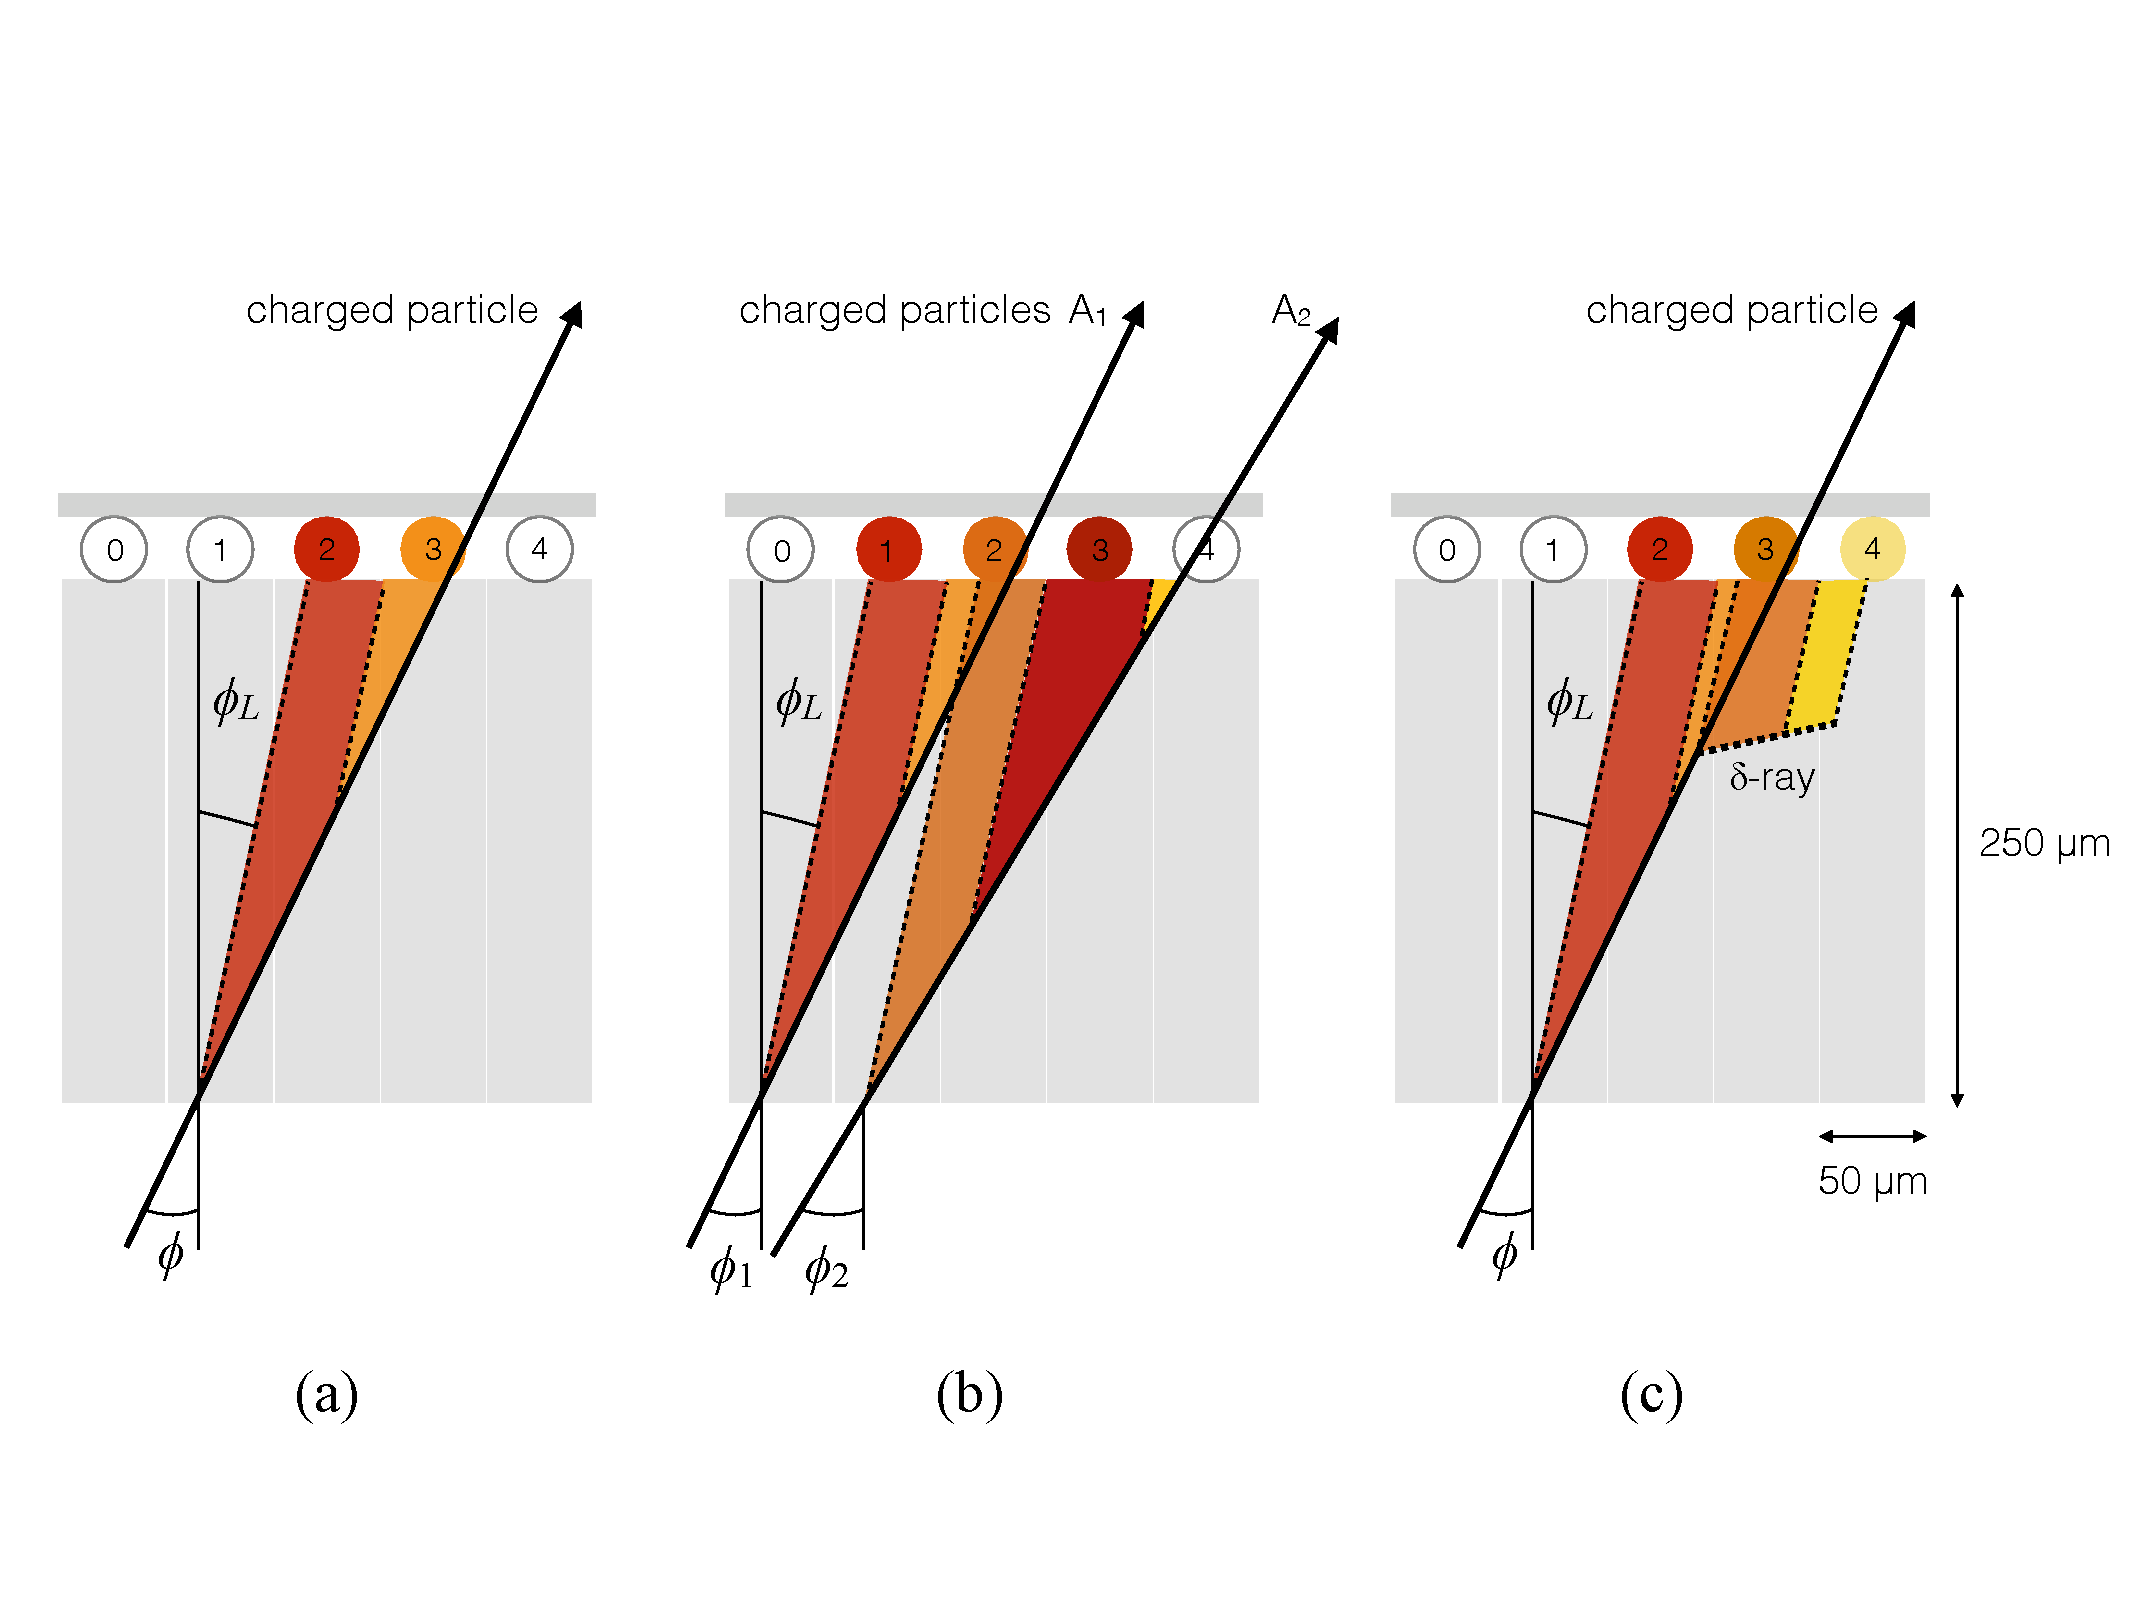
\includegraphics[width=\fullfig]{figures/pixel_cluster_types.pdf}
\caption{Examples of the clusters formed in a single layer of the pixel detector for (a) a single isolated particle, (b) two nearly-overlapping particles, and (c) a particle which emits a $\delta$-ray~\cite{pixel_nn}.}
\label{fig:pixel_cluster_types}
\end{figure}

A series of neural-networks analyzes the shape of the clusters to determine how many particles produced the cluster and to estimate the positions of each of the particles within the cluster.
These allow for an identification of clusters caused by more than one particle or by a particle that emits a $\delta$-ray.
In a high-density tracking environment, the multiple position outputs can be used as the locations of individual hits to allow reconstruction of tracks which almost overlap and with a much better separation than is possible without the splitting of individual clusters.

\subsection{Pixel dE/dx}
\label{sec:pixel_dedx}

A hit in the Pixel detector corresponds to the voltage generated from ionization current rising above a threshold value that is tuned to consistently record the passing of \acp{MIP}. 
A larger amount of charge deposited results in a larger voltage, and a larger signal remains above the threshold for a longer period of time.
The \ac{ToT} is read out of the Pixel detector, and can be used to provide a measurement of the charge deposited in each pixel.
The charge measurements from each of the pixels included in a pixel cluster are summed to form one charge measurement per layer of the pixel detector.
That charge measurement, combined with the angle of incidence of the track and the known sizes of each detector element, can be converted into a measurement of \dedx, the ionization energy deposited per unit distance, measured in \MeVgcm. 
The \ac{IBL} only has sixteen available values (4 bits) of \ac{ToT} to readout, compared to the 256 available values (8 bits) in the remaining pixel layers.
To help alleviate this lack of range, the \ac{IBL} also records if is in overflow: when the ionization is sufficient to generate a \ac{ToT} above the largest value that can be recorded in the 4 bits.

The measurements across multiple layers are combined to form an average value of \dedx for the track as a whole.
Depending on where a charge particle is produced, it will traverse four Pixel layers and create four clusters on average.
It can produce as few as two clusters in the Pixel detector if it passes through inactive modules, and as many as five if is in a region of the detector where multiple modules overlap.
To reduce the influence of the typical long Landau tails of the distribution of \dedx deposits~\cite{pdg}, the average is calculated as a truncated mean of these clusters.
The value measured in the \ac{IBL} is removed if it is in overflow, as the measured value is not reliable in that case.
If a track has five measurements in the pixel detector, the two highest cluster values are removed.
If a track has two, three, or four measurements in the pixel detector, only the single highest cluster value is removed.
The remaining values are averaged to form the pixel \dedx.

\subsection{Vertex Reconstruction}
\label{sec:vertices}

A vertex represents the intersection of multiple tracks and corresponds to the location of an interaction.
If at least two charged particles result from the interaction, the intersection of their resulting tracks reveals its position with high precision.
Vertices are divided into two groups, primary vertices which correspond to the actual proton-proton collisions, and secondary vertices which correspond to decays of short-lived particles or interactions with the detector. 
Primary vertices are particularly important, as they can provide a precise location for the interaction which generated the observed particles.
Understanding that location is crucial in understanding the geometry of the event.

Primary vertices are reconstructed by iteratively identifying seeds from reconstructed tracks~\cite{ATLAS-CONF-2010-069}.
Each track's extrapolated $z$ position at the beamline forms a seed, and nearby tracks are fitted using that position as a point along their trajectory.
The goodness of fit with that vertex is considered for each track, measured in $\chi^2$. 
The final position of the vertex is determined by a fit to all of the considered tracks, where the contribution from each track is weighted according to the $\chi^2$ compatibility with that vertex.
Any tracks from this procedure that are displaced by more than 7$\sigma$ from that vertex are removed from the fit and used to seed a new vertex.
This procedure is iterated until no additional vertices can be found.

This procedure is typically performed twice.
The first set of vertices is used to fit a profile for the beamspot, which indicates the position of the intersection of beams in that particular bunch crossing.
The fitted beamspot then provides a constraint for the second attempt to locate primary vertices, where both the track fitting and seeding of vertices are required to be consistent with interactions occurring within the beamspot.

% ----------------------------------------

\section{Electrons and Photons}
\label{sec:egamma}

Electrons are measured as both a charged particle track and energy deposits in the electromagnetic calorimeter.
Photons, on the other hand, leave energy deposits in the electromagnetic calorimeter but do not produce a corresponding track.
Because the electromagnetic interactions with the calorimeter of both photons and electrons produces more photons and electrons, the behavior in the calorimeter is very similar and their is significant overlap in the reconstruction techniques for each.

The reconstruction of a photon or an electron in the calorimeter is based on clustering algorithms which identify groups of energy deposits~\cite{PERF-2013-03, ATLAS-CONF-2014-032, ATLAS-CONF-2012-123}.
For this purpose, the entire electromagnetic calorimeter is subdivided into a grid of 200 by 256 towers in the $\eta$ and $\phi$ directions, respectively, where the individual grid units have a size of $\Delta\eta = 0.025$ and $\Delta\phi = 0.025$.
These towers correspond to individual cells in the middle, coarsest layer of the \ac{EM} calorimeter, and in the remaining layers the cells are grouped together cover the same area in $\eta-\phi$ space.
The clustering begins by finding seeds with a sliding-window algorithm based on the towers: a window of 3 by 5 towers is formed and translated until the sum of the energy within the window is maximized.
If that energy is above 2.5 \GeV, then that region becomes a seed.
The choice of 2.5 \GeV was chosen to compromise between maximizing reconstruction efficiency while minimizing fake electron seeds from electronic noise or soft hadrons from additional interactions.
The seeds are rejected if the energy measured in the hadronic calorimeter behind the seed is large, as this typically indicates a hadron rather than an electron or photon.

Next, the inner detector tracks within a cone of $\Delta R = 0.3$ are compared to the location and energy of the seed.
Tracks are matched to the cluster if the extrapolation of the track to the energy-weighted center in the middle layer of the \ac{EM} calorimeter falls within $\Delta\phi < 0.2$ in the direction of the curvature of the track or $\Delta\phi < 0.05$ in the direction opposite of the curvature of the track.
If the seed matches with a track that originated from a primary vertex, the combination of track and electromagnetic cluster is reconstructed as an electron.
If the seed matches with a track that did not originate from a primary vertex, then the electromagnetic cluster is reconstructed as a converted photon.
And if there is no corresponding track in the inner detector, than the cluster is reconstructed as a photon.

After classification, the final clustering of the energy in the \ac{EM} calorimeter calorimeter is performed.
The classification must be done first, as the expected size of the energy deposits in the calorimeter are different for electrons and photons.
In the barrel region, the final clusters for electrons are formed in rectangles of 3 towers in the $\eta$-direction and 7 towers in the $\phi$-direction.
This asymmetric window accounts for the curving of the produced charged particles only in the $\phi$ direction.
For photons, the size of the rectangle is 3 towers by 5 towers.
In the endcap region, all object types are clustered in rectangles of 5 towers by 5 towers, as the effect of the magnetic field curvature is less pronounced in this region.
The sum of the energies in these clusters provide the final energy measurement for the electron or photon.

\subsection{Photon Identification}

The original requirement for constructing a photon cluster, a significant energy deposit in the electromagnetic calorimeter without a corresponding track or energy deposits in the hadronic calorimeter, is already effective in identifying photons.
However, there is a significant background for prompt photon production from the decays of pions, $\piz \rightarrow \gamma\gamma$.
These can be identified using the shape of the cluster in the narrow $\eta$ granularity in the first layer of the \ac{EM} calorimeter.

\subsection{Electron Identification}

Prompt electrons have a number of backgrounds, such as secondary electrons from hadron decays or misidentified hadronic jets, that can be rejected using additional information from the \ac{EM} calorimeter and the inner detector.
The most basic level of electron identification, referred to as Loose, makes requirements on the shower shapes in the high granularity first layer of the \ac{EM} calorimeter as well as the quality of the inner detector track.
It also requires a good match between the track and the calorimeter energy deposits and a small fraction of energy in the hadronic calorimeter behind the electromagnetic cluster.
\ac{ATLAS} defines several additional working points, including Medium and Tight, which provide progressively lower background rates for electrons by imposing additionally strict requirements on the above variables as well as new requirements like the impact parameter of the inner detector track or the comparison of the cluster energy to the momentum in the inner detector.

% ----------------------------------------

\section{Muons}
\label{sec:muons}

Muons produced in \ac{ATLAS} first traverse the inner detector and leave behind a track as described in Section~\ref{sec:tracks}.
The muon then passes through the calorimeter, leaving behind a small, characteristic amount of energy, and then passes through the muon spectrometer where it produces hits in the \acp{MDT} or \acp{CSC}.
Muon tracks are formed from local segments of hits in each layer of the \acp{MDT} or \acp{CSC}, and then the final muon spectrometer track is formed by combining the two local segments~\cite{PERF-2015-10}.
When a track is reconstructed in both the inner detector and the muon spectrometer, the track is refitted to include the hits in both the inner detector and the muon spectrometer, and forms a combined muon.

In a few regions of the detector, a muon may fail to leave behind both a complete inner detector and muon system track.
For a very small fraction of the acceptance of the muon system, there is only one layer of muon chambers and a global muon system track is not formed.
In this case, as long as the track in the inner detector exists and geometrically matches to a segment, a segment-tagged muon is formed using momentum measurements from the inner detector.
In the region where the muon system has coverage but the inner detector does not, $2.5 < |\eta| < 2.7$, a stand-alone muon is formed which uses only information from the muon system.
And for muons produced within one of the few holes in the muon system, including $|\eta| < 0.1$, the characteristic energy deposits in the calorimeter can be used to tag an inner detector track as a calo-tag muon.
These additional categories are used to achieve high efficiency over a larger range of acceptance, but the combined muons are the most reliable.

\subsection{Muon Identification}

The various types of muons are incorporated into three working points: Loose, Medium, and Tight, which reflect the increasing muon purity for each of the selections definitions.
Tight muons include only combined muons with a good track fit quality and momentum resolution and at least two hits in a precision muon system layer.
Medium muons include those in tight as well as combined muons with one precision hit and one precision hole, where hole is defined in the same way as in Section~\ref{sec:tracks}.
The medium working point also includes stand-alone muons with $|\eta| > 2.5$ and at least two hits in precision layers.
And finally the loose working point includes both medium and tight muons, but additional includes segment-tagged and calo-tagged muons in the region $|\eta| < 0.1$.

% ----------------------------------------

\section{Jets}
\label{sec:jets}

A jet does not directly correspond to a physical particle, unlike all of the reconstructed objects described above, but instead tries to capture the conical cascade of particles produced in the hadronization of a quark or gluon from the proton-proton collision.
The hadronization process creates a very large number of collimated particles, with a high enough density that individually reconstructing all of the produced particles in the calorimeter is not possible within \ac{ATLAS}.
However most analyses are interested only in the kinematics of the particle which produced the cascade, rather than the individual products.
Therefore, jets are a useful tool to measure the combined energy and direction of the ensemble of products and thus represents the kinematics of the original.
Jet algorithms are very generic and can be used to group together a number of types of objects to form aggregate representations.
For example, truth particles in simulation can be grouped in truth jets, or tracks from the inner detector can be grouped together to form track jets. 
This section, however, will focus on calorimeter jets which take topoclusters of energy deposits in the calorimeter as inputs and produce a combined object which represents the energy measured by the calorimeter and the location where it was deposited.

\subsection{Topological Clustering}

Hadrons often deposit their energy into multiple individual cells in both the electromagnetic and hadronic calorimeters.
The purpose of topological clustering is to group cells in all three dimensions into clusters that represent a single energy deposit.
The procedure must be robust enough to reject noise fluctuations in the cell energy measurements that can come from both electronic noise and additional low energy particles produced in pileup activity.
The background level of calorimeter noise is called \signoise, and is an important component of the topological clustering.

The topological clusters are formed in a three step process called the 4-2-0 threshold scheme, which uses three energy thresholds to build up a cluster from cells~\cite{PERF-2014-07}.
First, any cells with a measured energy above 4\signoise are identified as seed cells. 
The cells adjacent to the seed cells with a measured energy above 2\signoise are called secondary cells.
All of the cells which are adjacent to a secondary cell with $E_\mathrm{cell} > 2\signoise$ are also labeled secondary cells.
Tertiary cells are those immediately adjacent to a seed or secondary cell with a measured energy above zero.
Adjacency in this sense is defined in three dimensions, cells are adjacent if they are neighbors within a layer but also if they have the same $\eta-\phi$ coordinates but are in adjacent layers or even in an adjacent layer in another calorimeter.

From these definitions, clusters are built by resolving the seeds in order of significance, the ratio $E_{\mathrm{cell}}/\signoise$.
All adjacent secondary cells to the highest significance seed are added to that seed's topocluster, and any of those cells which would also have qualified as seeds are removed from the list of seeds.
Once all of the secondary cells have been added, the tertiary cells are then added to that cluster as well.
This procedure is then iterated until no seeds remain, forming the first round of topoclusters.

It is also useful to split topoclusters into multiples if local maxima are present within the topocluster, as clusters produced by multiple nearby particles can merge.
The splitting process begins by finding local maxima cells in the middle layer of the calorimeters with a minimum energy of 500 \MeV and at least four neighboring secondary cells.
These requirements reduce the likelihood to split a cluster due to random fluctuations, as the middle layers provide the most reliable energy measurements.
Cells between two local maxima can then be shared between two clusters to account for overlapping contributions from two particles. The energy sharing is weighted by the energy of each cluster as well as the distance of the cell to the centroid of that cluster.

The energies of all the cells in the cluster are then summed together to form the energy of that cluster.
The energy needs to be corrected for the various losses expected in the calorimeter, as described in Section~\ref{sec:calorimetry}.
The simplest correction, scaling the measured energy by the sampling fraction, brings the cluster energies to the \ac{EM} scale.
It is called the \ac{EM} scale because it accurately describes the energy of electromagnetic showers.

Another scale is defined to improve accuracy for hadronic processes, the \ac{LCW} scale, that helps to correct for the expected variations in hadronic energy deposits.
The \ac{LCW} correction first determines if the shower is hadronic or electromagnetic, based on the depth of the shower and the cluster energy density.
For hadronic showers, the energy is corrected for calorimeter non-compensation, an effect which reduces the measured energy of hadronic showers because some of the energy goes into invisible processes like the break up of nuclei.
All clusters are then corrected for energy that may be deposited in uninstrumented regions in that cluster's location in the calorimeter, and they are also corrected with an estimate of how much energy falls outside the extent of the cluster based on its shape and the deposit type.

\subsection{Jet Algorithms}
Using the topological clusters as inputs, a jet algorithm groups them together into a collection of adjacent energy deposits that is intended to correspond to a single process~\cite{ATL-PHYS-PUB-2015-036}.
Jet algorithms need a few key characteristics to be usable for physics analysis.
First, the jets produced by the algorithm should have little dependence on the addition of soft particles to the event (infrared safety), as a negligible addition of energy should not significantly modify the event topology.
Similarly, the jets produced by the algorithm should also not significantly depend on mostly collinear splitting of an input particle (collinear safety); that is, a single quark replaced by two, parallel quarks with half the original's momentum should not change the resulting jets, which are intended to capture only the properties of the aggregate and not those of individual particles.
And finally the algorithm needs to be sufficiently simple and fast to be used for the large rate of collected proton-proton collisions on \ac{ATLAS}.

The most commonly used algorithm on \ac{ATLAS} that satisfies these requirements is called the anti-$k_t$ algorithm, and is discussed in further detail in Reference~\cite{antikt}.
The anti-$k_t$, in brief, relies on iteratively combining the input objects that are closest together, where closest is defined by a particular distance metric, $d_{i,j}$, where the index $i$ represents the combination constructed so far and $j$ is an additional object being considered.
The combinations stop when the closest remaining object is the beam itself, where the distance to the beam is called $d_{i,B}$. 
An entire class of algorithms follows this procedure with the following distance metrics

\begin{align}\label{eq:antikt}
d_{i,j} &= \min(k_{ti}^{2p}, k_{tj}^{2p}) \frac{\Delta_{ij}^2}{R^2} \\
d_{i,B} &= k_{ti}^{2p}
\end{align}

where $\Delta_{i,j} = (y_i - y_j)^2 + (\phi_i - \phi_j)^2$, $k_{ti}$ is the transverse momentum of the object, $y$ is the rapidity, and $p$ is a parameter of the algorithm.
Anti-$k_t$ is the particular case where $p = -1$, and is a choice that results in an algorithm that is both infrared and collinear safe.

The algorithm is repeated until there are no input objects remaining, which results in a series of jets. 
Each jet has a complete four momentum from the combination of its input clusters, where the combinations assume a mass of zero.
The jet energies then need to be calibrated to attempt to match the energy of the object which produced the jet.

\subsection{Jet Energy Scale}
\label{sec:reco_jes}

Though the \ac{LCW} scheme attempts to correct the topoclusters to reflect the true deposited energy, the correction does not fully account for energy lost within the calorimeters.
Because of these effects, the original reconstructed jet energy does not reflect the true energy of the particle which initiated the jet.
Therefore it is necessary to additionally correct the reconstructed jet itself, in addition to the corrections on the inputs.
This correction is referred to as the \ac{JES}, which combines several individual steps of calibration~\cite{ATLAS-CONF-2015-002}.

The first calibration step corrections the direction of the jet to ensure that it points back to the primary vertex.
Next, the energy of the jet is corrected for pileup by subtracting the expected contribution from pileup based on the momentum, $\eta$, and area of the jet as well as the number of reconstructed vertices and expected number of interactions per crossing.
The largest single correction is the absolute $\eta$ and scale correction, where the jet energy and pseudorapidity is corrected to attempt to match the energy and pseudorapidity of the parton which produced it.
This correction is measured in simulation by comparing the reconstructed jet energies to the energy of the truth particle which produced it.
However the simulation is not relied on alone to estimate this correction, and an additional step applies an additional energy correction based on in-situ measurements in data.
These corrections come from various techniques which measure jet energies indirectly by balancing them with other, well-measured objects.
In the central region ($|\eta| < 1.2$), jets are balanced against photons and the leptonic decays of Z bosons and high momentum jets ($p_T > 210$ GeV) are also balanced against multiple smaller jets in multijet events.
Jets at larger pseudorapidities, above $|\eta| = 1.2$, are calibrated by balancing with lower pseudorapidity jets.

These steps introduce a number of systematic uncertainties, referred to as the \ac{JES} uncertainty.
The largest of these comes from the in-situ measurements, which are statistically limited in measuring high momentum and high pseudorapidity jets.
The total, fractional \ac{JES} uncertainty is shown as a function of $p_T$ in Figure~\ref{fig:reco_jesunc}.
The uncertainty falls to a minimum value of just over 1.0\% around a few hundred \GeV, and rises again at high momentum because of the difficulty of measuring jet balance in data above 2-3 \TeV.
The uncertainty is also minimized at low $|\eta|$, and grows at large $|\eta|$ again where making in-situ measurements is difficult.
This technique does not actually provide a measurement of the uncertainty for the highest energy jets, above 3 \TeV, because there are not enough measured data events to provide them.
An alternative method for deriving the \ac{JES} and \ac{JES} uncertainty that can be used even for very high $p_T$ jets will be discussed in Chapter~\ref{ch:jes}.

\begin{figure}
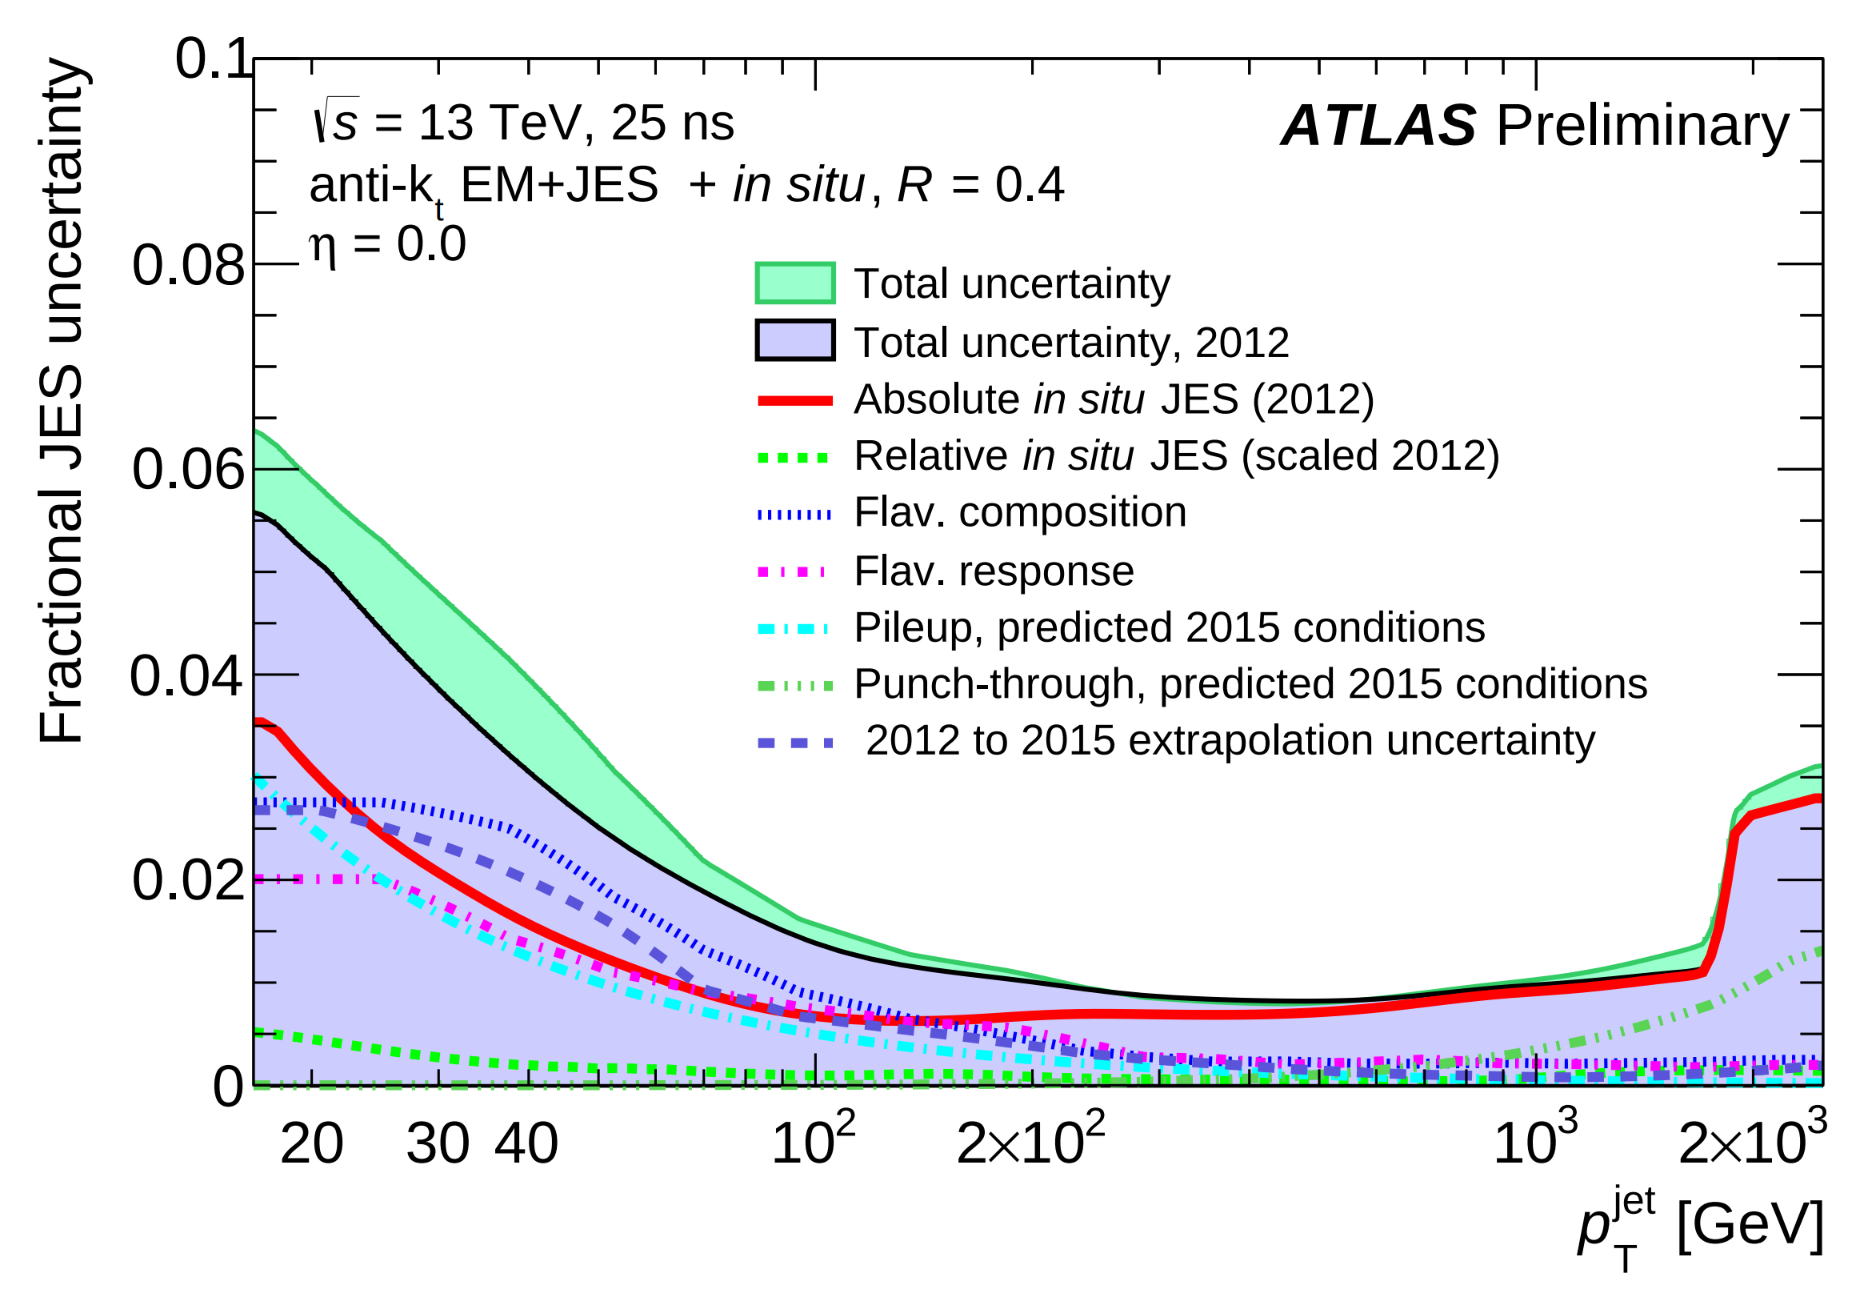
\includegraphics[width=\fullfig]{figures/reco_jes_pt.png}
\caption{The total, fractional \ac{JES} uncertainties estimated for 2015 data as a function of jet $p_T$.}
\label{fig:reco_jesunc}
\end{figure}

% ----------------------------------------

\section{Missing Transverse Energy}
\label{sec:missing_energy}

Among stable \ac{SM} particles, only the neutrino cannot be directly measured in the \ac{ATLAS} detector. 
Because the neutrino carries neither electric nor color charge, it is very unlikely to interact with the tracking detectors or the calorimeters, and instead passes through the detector completely unobserved.
Some particles which have been conjectured to exist, like the \ac{LSP} in many \ac{SUSY} models, would also have the same behavior.
Therefore, it is important for \ac{ATLAS} to provide some way to assess the momentum carried away by a neutral, colorless particle.
This can be accomplished through a measurement of missing energy in the transverse direction, or \met, which quantifies the momentum imbalance of the observed particles.
From the conservation of momentum and the lack of the initial momentum in the transverse plane in the proton-proton collisions, any imbalance of momentum can be inferred to be carried away by an unmeasured particle.

\met is more precisely defined as the magnitude of the vector sum of the $(p_x,p_y)$ components of each observed object's momentum.
The definition is simple, but there can be significant complexity in defining the inputs.
As of Run 2, \ac{ATLAS} uses a common algorithmic approach to carefully calculate missing energy, but each analysis is free to define it's own inputs.
For the analysis discussed throughout this thesis, the missing energy inputs consist of the electrons, photons, muons, and jets discussed in the previous sections, in addition to a track-based soft term.

To produce the most precise measurement of \met, it is important to use the best representation of the momentum of each of the input objects, which can often be reconstructed as multiple different types in a single event.
For example, an electron can be reconstructed separately as an electron (Section~\ref{sec:egamma}) and a jet (Section~\ref{sec:jets}), but the electron representation has the highest precision for reconstructing the true electron momentum.
To ensure no duplications in the \met definition, the inputs are collectively considered for overlap removal.
Only the most precise object type is kept for objects that fall within a cone of $\Delta R < 0.2$ for pairs of electrons and jets and a cone of $\Delta R < 0.4$ for other pair types.

The fully reconstructed objects do not include all of the energy within the events, as some clusters do not enter into a jet and some tracks are not classified as electrons or muons.
These momentum carried by these objects is accounted for in a soft-term, which tallies all of the energy carried by the particles too soft to form separate objects.
The track soft term uses only tracking information to estimate the contribution of soft objects, and does so by vectorially summing the momentum of all well-reconstructed tracks with momentum above 400 \MeV.

All of these contributions together give a single \met value for a given event.
The direction of that missing energy is taken as opposite the vector sum of all the constituents, to correspond to the momentum an invisible particle would have to have to make the event balanced.
Depending on the context, this missing energy can be considered the energy of a neutrino or an \ac{LSP}, with a large missing energy being a common signal criteria for searches for new physics.

% ----------------------------------------
